\documentclass[a4paper]{report}

%====================== PACKAGES ======================

\usepackage[french]{babel}
\usepackage[utf8x]{inputenc}
%pour les commentaires
\usepackage{verbatim}
%pour gérer les positionnement d'images
\usepackage{float}
\usepackage{amsmath}
\usepackage{graphicx}
\usepackage{url}
%pour les informations sur un document compilé en PDF et les liens externes / internes
\usepackage{hyperref}
%pour la mise en page des tableaux
\usepackage{array}
\usepackage{tabularx}
%pour utiliser \floatbarrier
%\usepackage{placeins}
%\usepackage{floatrow}
%espacement entre les lignes
\usepackage{setspace}
%modifier la mise en page de l'abstract
\usepackage{abstract}
\usepackage{}
%police et mise en page (marges) du document
\usepackage[T1]{fontenc}
\usepackage[top=2cm, bottom=2cm, left=2cm, right=2cm]{geometry}
%Pour les galerie d'images
\usepackage{subfig}
%Pour les graphes
\usepackage{pgfplots}
\pgfplotsset{width=10cm,compat=1.9}
%\usepgfplotslibrary{external}
%\tikzexternalize

%====================== INFORMATION ET REGLES ======================

%rajouter les numérotation pour les \paragraphe et \subparagraphe
\setcounter{secnumdepth}{4}
\setcounter{tocdepth}{4}

\hypersetup{
colorlinks = true,
linkcolor=black ,						% Information sur le document
pdfauthor = {Premier Auteur,
			Deuxième Auteur,
			Troisième Auteur,
    		Quatrième Auteur},			% Auteurs
pdftitle = {Nom du Projet -
			Sujet du Projet},			% Titre du document
pdfsubject = {Mémoire de Projet},		% Sujet
pdfkeywords = {Tag1, Tag2, Tag3, ...},	% Mots-clefs
pdfstartview={FitH},					% ajuste la page à la largueur de l'écran
%pdfcreator = {MikTeX},% Logiciel qui a crée le document
%pdfproducer = {}} % Société avec produit le logiciel
}
%======================== DEBUT DU DOCUMENT ========================

\begin{document}

%régler l'espacement entre les lignes
\newcommand{\HRule}{\rule{\linewidth}{0.5mm}}

%page de garde
\begin{titlepage}
\begin{center}

% Upper part of the page. The '~' is needed because only works if a paragraph has started.

\includegraphics[width=0.35\textwidth]{./logo}~\\[1cm]
\textsc{\LARGE Université Cheikh Anta Diop }\\[1.5cm]
\textsc{\LARGE Ecole Supérieure Polytechnique de Dakar }\\[1.5cm]

\textsc{\Large }\\[0.5cm]

% Title
\HRule \\[0.4cm]

{\huge \bfseries Systèmes Multi Agents\\
Etude de cas \\[0.4cm] }

\textsc{\Large }\\[0.5cm]²
\HRule \\[1.5cm]

% Author and supervisor
\begin{minipage}{0.4\textwidth}
\begin{flushleft} \large
\emph{Auteurs:}\\
Papa Latyr \textsc{Mbodj}\\
Cheikh Ahmet Tidjane \textsc{Sankare}\\
\end{flushleft}
\end{minipage}
\begin{minipage}{0.4\textwidth}
\begin{flushright} \large
\emph{Superviseur:} \\
Pr Alassane \textsc{Bah}
\end{flushright}
\end{minipage}

\vfill

% Bottom of the page
{\large \today}

\end{center}
\end{titlepage}

%page blanche
\newpage
~
%ne pas numéroter cette page
\thispagestyle{empty}
\newpage

\renewcommand{\abstractnamefont}{\normalfont\Large\bfseries}
%\renewcommand{\abstracttextfont}{\normalfont\Huge}
\renewcommand{\abstractname}{Introduction}

\begin{abstract}
\hskip7mm

\begin{spacing}{1.3}

Afin d’appliquer les notions enseignées en Cours de Systèmes Multi Agents, nous avons eu à réaliser une étude de cas avec GAMA,un environnement de développement orienté modélisation et simulation de systèmes à base d'agents. Cet étude de cas concerne une \textbf{\textit{exploitation d'un territoire minier par une population de robots}}. Les robots doivent trouver tous les minerais présents dans le territoire et les amener à une base.\\
L'étude de cas est décliné en deux versions : une première version avec des robots réactifs et une deuxième version avec des robots cognitifs. Nous avons structuré notre rapport de la façon suivante :
Tout d'abord, dans une première partie nous faisons une spécification générale dans laquelle nous fixons les définitions de chacun des éléments manipulés dans notre étude de cas. Puis dans une seconde partie, nous présentons la première version du robot, le robot réactif. Ensuite, dans une troisième partie, nous déclinerons le robot cognitif. Puis nous ferons des test de sensibilité et comparaisons des deux versions avant de finir par une conclusion.

\end{spacing}
\end{abstract}



\tableofcontents


\setcounter{page}{0}
%ne pas numéroter le sommaire

\newpage

%espacement entre les lignes d'un tableau
\renewcommand{\arraystretch}{1.5}

%====================== INCLUSION DES PARTIES ======================

~
\thispagestyle{empty}
%recommencer la numérotation des pages à "1"
\setcounter{page}{0}
\newpage

\chapter{Spécifications}

%Intro\footnotemark\\
%note en bas de page


\section{Environnement}

Notre environnement est une grille carrée de 20 lignes et 20 colonnes donc 400 cellules de type "test\_grid". A partir de chaque cellule, il est possible d'obtenir la liste de ses 4 voisins les plus proches; celui de gauche, celui de droite, celui d'en haut et celui d'en bas. Toutes les interactions se font dans cet environnement.\\

%inclusion d'une mage dans le document
\begin{figure}[!h]
\begin{center}
%taille de l'image en largeur
%remplacer "width" par "height" pour régler la hauteur
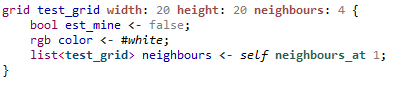
\includegraphics{code/test_grid}
\end{center}
%légende de l'image
\caption{Définition d'une grille de l'environnement}
\end{figure}

%Contenu de la note précédemment marquée avec \footnotemark
%\footnotetext{Note bas de page "intro"}


\section{Minerais}

Pour représenter les minerais dans l'environnement, nous prenons aléatoirement autant de cellules que de minerais que nous voulons représenter. Afin de faire de ces cellules des mines, nous leur attribuons un état miné pour de dire qu'elles contiennent des mines. Aussi, nous colorons les cellules minées en noir.

%inclusion d'une mage dans le document
\begin{figure}[!h]
	\begin{center}
		%taille de l'image en largeur
		%remplacer "width" par "height" pour régler la hauteur
		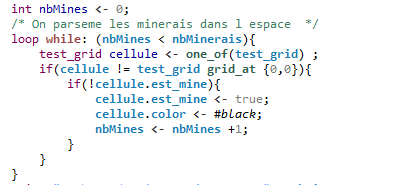
\includegraphics{code/minerais}
	\end{center}
	%légende de l'image
	\caption{Dissémination des minerais}
\end{figure}

\newpage

\section{Base}

Elle représente l’agent passif qu’est la base ici, c’est a dire qu’elle ne fait rien et ne sert ici que de cible de dépôt pour les minerais collectés. Elle sauvegarde la référence vers la cellule de grille dans laquelle elle se trouve. 

\begin{figure}[!h]
	\begin{center}
		%taille de l'image en largeur
		%remplacer "width" par "height" pour régler la hauteur
		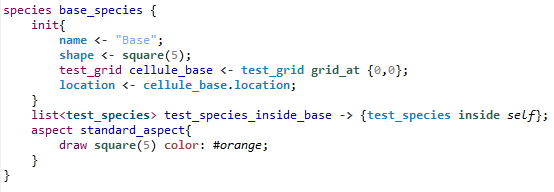
\includegraphics{code/base}
	\end{center}
	%légende de l'image
	\caption{Base de dépôt des minerais}
\end{figure}

\section{Robot réactif}

C’est notre type de robot de base. Il représente des robots réactifs, c’est a dire qui entreprennent des actions qu'en fonction de leur environnement sans aucun apprentissage.  Ils n’ont aucune possibilité de connaitre à l'avance la localisation de la base de dépôt des minerais. Pour trouver la base, ils se déplacent aléatoirement de voisins en voisins jusqu'à’à se trouver à la base Le robot a un nom, sa position actuelle dans l'environnement ainsi que le minerai qu'il porte (potentiellement). Il a aussi un objectif qui peut être soit de chercher des minerais, soit de prendre un minerai, soit d'aller a la base, soit de déposer un minerai a la base.\\
Lorsqu'on l'introduit dans l'environnement lors de l'initialisation, son objectif est de chercher un minerai. Des qu'il en trouve, son objectif devient d'aller a la base. Une fois a la base, il doit y déposer le minerai. Ses objectifs sont atteints à l'aide de réflexes\footnotemark.\\

Dans le cas de notre robot réactif, les réflexes définis sont les suivants:
\begin{itemize}
\item \textbf{chercher\_minerai} qui permet au robot de rechercher des minerais dans l'environnement;
\item \textbf{prendre} qui permet au robot de prendre un minerai trouvé;
\item \textbf{aller\_base} qui permet au robot d'aller à la base;
\item \textbf{deposer} qui permet au robot de déposer un minerai dans la base.
\end{itemize}

\begin{figure}[!h]
	\begin{center}
		%taille de l'image en largeur
		%remplacer "width" par "height" pour régler la hauteur
		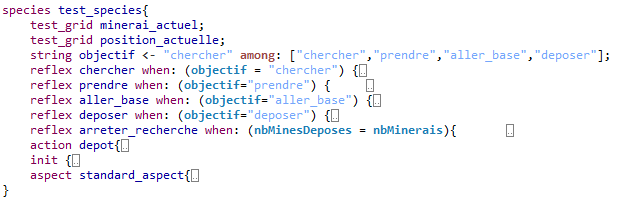
\includegraphics{code/robot_reactif}
	\end{center}
	%légende de l'image
	\caption{Robot réactif}
\end{figure}

\footnotetext{Les réflexes sont des ensembles d'instructions qui s'exécutent après chaque cycle du robot (pas de temps). Elles représentent ainsi les compétences spécifiques des agents et correspondent aux opérations d'une classe ou aux activités dans un diagramme d'activité. }

\section{Robot cognitif }
C’est notre deuxième type de robot. Il s'agit d'une version améliorée du robot réactif. Ce robot a les mêmes réflexes que le premier type de robot. La différence se trouve au niveau du réflexe aller\_base qui est faite ici de façon plus intelligente. En effet, tout comme le robot réactif, le robot cognitif n'a aucune connaisance de l'emplacement de la base à l'avance. Mais, une fois après y être allé, il mémorise cet emplacement. Cela fait qu'après, il ne recherche plus la base mais y va directement en prenant le chemin le plus court.
\begin{figure}[!h]
	\begin{center}
		%taille de l'image en largeur
		%remplacer "width" par "height" pour régler la hauteur
		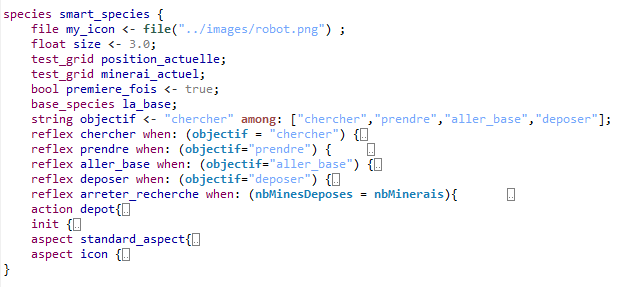
\includegraphics{code/robot_cognitif}
	\end{center}
	%légende de l'image
	\caption{Robot cognitif}
\end{figure}


\chapter{Première Version : Robot Réactif}



\section{Diagramme de Classes}

Le diagramme de classe est censé représenté la structure statique d'un système. Seulement comme dans GAMA tout est agent, les classes que nous manipulerons ici ne représentent en fait que des agent formalisés selon UML. Elles dérivent donc toutes de la classe "agent" nativement définie dans la documentation de GAMA. Nous ne représenterons pas cette classe dans nos diagrammes ici. 
Ci-dessous le diagramme de classe du modèle avec Robots Réactifs. 

\begin{figure}[h!]
	\begin{center}
		%taille de l'image en largeur
		%remplacer "width" par "height" pour régler la hauteur
		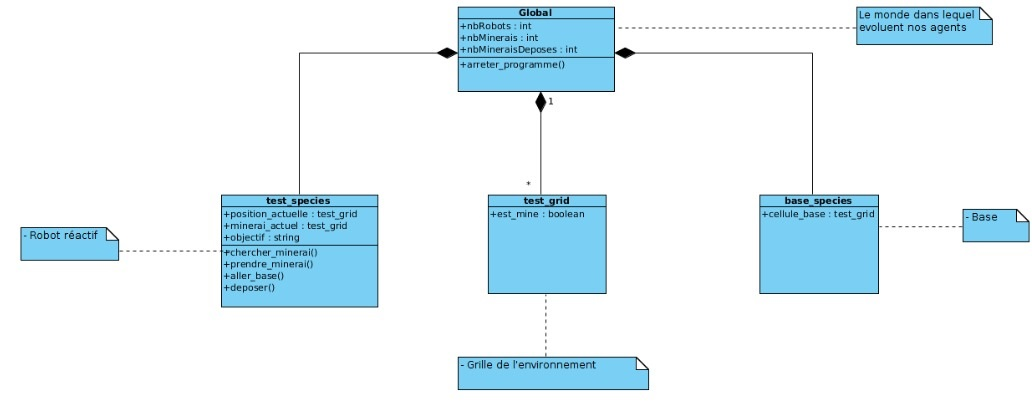
\includegraphics[width=500pt]{diagrammes/diagramme_classe_reactif}
	\end{center}
	%légende de l'image
	\caption{Diagramme de classe du robot réactif}
\end{figure}


Dans ce diagramme nous avons:

\begin{description}
	\item[Le Monde "global"] Il représente l'environnement dans lequel s'exécute la simulation. Il est lui même un agent et sert de conteneur a tous les autres agents du modèle, ce qui justifie la relation de composition qu'il partage avec toutes les autres classes. Comme son nom l'indique, il contient l'ensemble des variables et configurations globales du modèle et des expérimentations que nous ferons. 
	
	\item[La grille (les Cellules) "test\_grid"] Ce sont les cellules de la grille dans laquelle notre simulation se déroule. Chacune d'entre elle est dotée d'un attribut additionnel "est\_mine" qui permet de connaitre si la zone recouverte par la cellule contient ou non un minerai.
	
	\item[la Base "base\_species"] c'est l'agent qui représente la base de stockage des minerais. Il est associé à une des cellules de la grille choisie arbitrairement (ici cellule de la première ligne et de la premiere colonne) avec qui elle partage ainsi la même position. 
	
	\item[Les Robots Réactifs "test\_species"] C'est notre Robot collecteur, il est réactif mais pas "intelligent" puisqu'il n'a aucun moyen de savoir à priori où se trouve la base. Tout ce qu'il sait faire c'est se déplacer aléatoirement de voisins en voisins jusqu'à ce qu'il trouve la base dans sa zone de perception (cellule actuelle + cellules voisines).
\end{description}

\section{Diagramme d'Activités}

\begin{figure}[!h]
	\begin{center}
		%taille de l'image en largeur
		%remplacer "width" par "height" pour régler la hauteur
		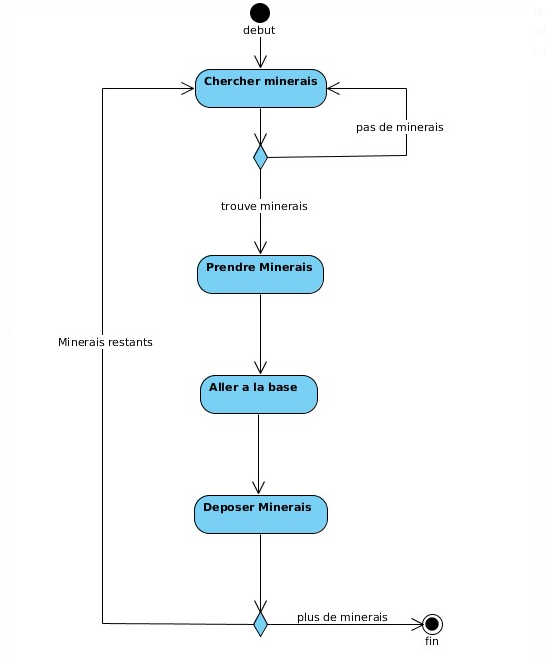
\includegraphics{diagrammes/diagramme_activites_reactif}
	\end{center}
	%légende de l'image
	\caption{Diagramme d'activités du robot réactif}
\end{figure}

Voici le diagramme d'activités du robot réactif. Ces activités correspondent à des réflexes de nos agents. Nous allons détailler chacune de ces activités.

\newpage

\subsection{Recherche de minerai [Chercher Minerais]}

Dans cette étape du scénario le robot vérifie d'abord si la cellule de grille (qui correspond à une zone) dans laquelle 
il se trouve contient un minerais. Sinon il cherche si les cellules voisines en contiennent. Si ni la cellule actuelle ni aucune de ses voisines ne contiennent de minerais alors le robot se déplace aléatoirement dans l'une des cellules voisines de la cellule actuelle pour y exécuter le même traitement au prochain pas de temps (cycle). Dans le cas contraire (il trouve un minerais) il passe à l'étape de collecte du minerais. \\
Cette étape du scénario est implémentée de la façon suivante : 
\begin{figure}[!h]
	\begin{center}
		%taille de l'image en largeur
		%remplacer "width" par "height" pour régler la hauteur
		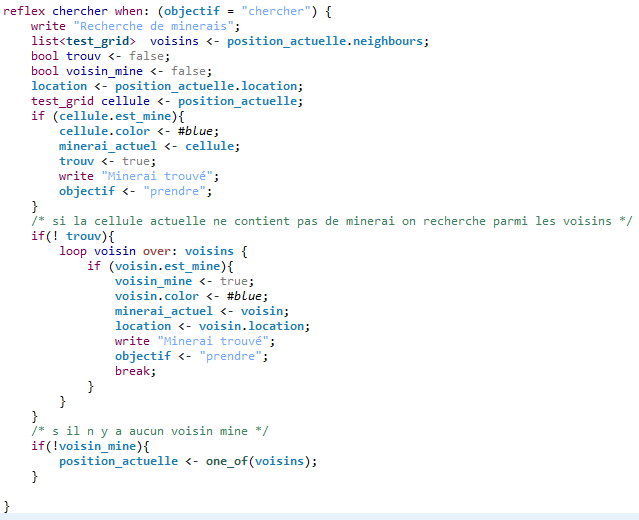
\includegraphics{code/chercher}
	\end{center}
	%légende de l'image
	\caption{Réflexe chercher}
\end{figure}

\subsection{Prise de minerai [Prendre Minerai]}

Cette étape ne se déclenche que quand le robot trouve un minerais dans l'une des cellules qu'il vient d'explorer. Durant cette etape le robot correspond a la collecte de minerais presénts dans la zone explorée. Cela correspond dans notre simulation à la modification d'un certain nombre d'attributs du robot et de la cellule de grille dans laquelle le minerais a été trouvé.\\
\newpage
Cette étape du scénario est implémentée de la façon suivante : 
\begin{figure}[!h]
	\begin{center}
		%taille de l'image en largeur
		%remplacer "width" par "height" pour régler la hauteur
		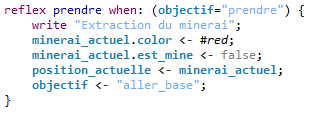
\includegraphics{code/prendre}
	\end{center}
	%légende de l'image
	\caption{Réflexe prendre}
\end{figure}

\subsection{Acheminement des minerais vers la base [Aller a la Base]}

Cette étape correspond à l'ensemble des déplacements aléatoires que le robot fait de voisins en voisins afin de trouver la base et d'y déposer le minerais collecté.\\ 
Cette étape du scénario est implémentée de la façon suivante : 
\begin{figure}[!h]
	\begin{center}
		%taille de l'image en largeur
		%remplacer "width" par "height" pour régler la hauteur
		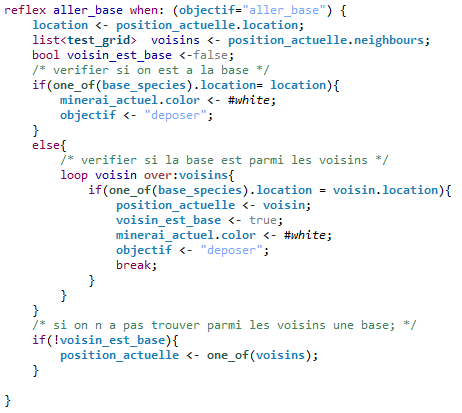
\includegraphics{code/aller_base_reactif}
	\end{center}
	%légende de l'image
	\caption{Réflexe aller\_base}
\end{figure}


\subsection{Dépôt de minerai}

Cette étape se déclenche une fois que le robot arrive a la base avec du minerais collecté. Elle correspond aussi (dans notre simulation) a la modification d'un ensemble d'attributs du robot qui montre que le dépôt a été bien fait et que le robot est à présent vide et prêt à aller rechercher d'autres minerais s'ils existent.\\
\newpage
Cette étape du scénario est implémentée de la façon suivante : 
\begin{figure}[!h]
	\begin{center}
		%taille de l'image en largeur
		%remplacer "width" par "height" pour régler la hauteur
		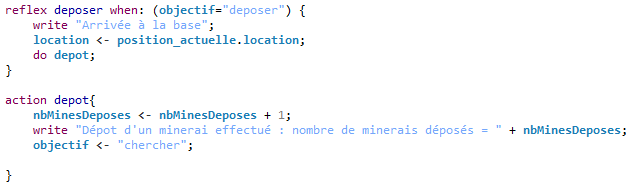
\includegraphics{code/deposer}
	\end{center}
	%légende de l'image
	\caption{Réflexe deposer}
\end{figure}


\subsection*{} 
Dans le diagramme d'activités ci-dessus les activités correspondent aux étapes que nous avons définies précédemment. Les seules nouveautés sont les deux nœuds de conditions:
\begin{itemize}
	\item La première se fait après l'étape "Chercher Minerais" et permet de tester si le robot a trouver un minerais dans sa zone de perception et ainsi 
	decider de s'il doit collecter et aller à la base ou tout simplement retourner à l'étape de recherche dans une autre zone de perception voisine.
	
	\item La seconde permet tester s'il existe encore des minerais dans l'environnement. Si c'est le cas le robot reprend tout le cycle d'activités à partir du début. Dans le cas contraire il s'arrête tout simplement.
\end{itemize}

 
\chapter{Deuxième Version : Robot Cognitif}


Les robots  cognitifs sont tout d'abord des robots interactifs. La seule différence c'est qu'ils sont dotés de la capacité de se mémoriser la position de la base après l'avoir trouvé. Cette différence sera d'ailleurs la seule que l'on pourra remarquer dans les diagrammes des deux cotés.


\section{Diagramme de Classes}

Le diagramme de classe aussi ne contient pas beaucoup de changements pour les robots cognitifs. En plus du diagramme de classe précédent, nous avons une nouvelle classe "smart\_species" (robot cognitif) qui hérite de la classe "test\_species" (robot réactif) avec un seul nouvel attribut: "la\_base". En effet il contient les coordonnées de la base permettant ainsi au robot de pouvoir s'y diriger directement. La méthode aller\_base() y est redéfinie.

\begin{figure}[!h]
	\begin{center}
		%taille de l'image en largeur
		%remplacer "width" par "height" pour régler la hauteur
		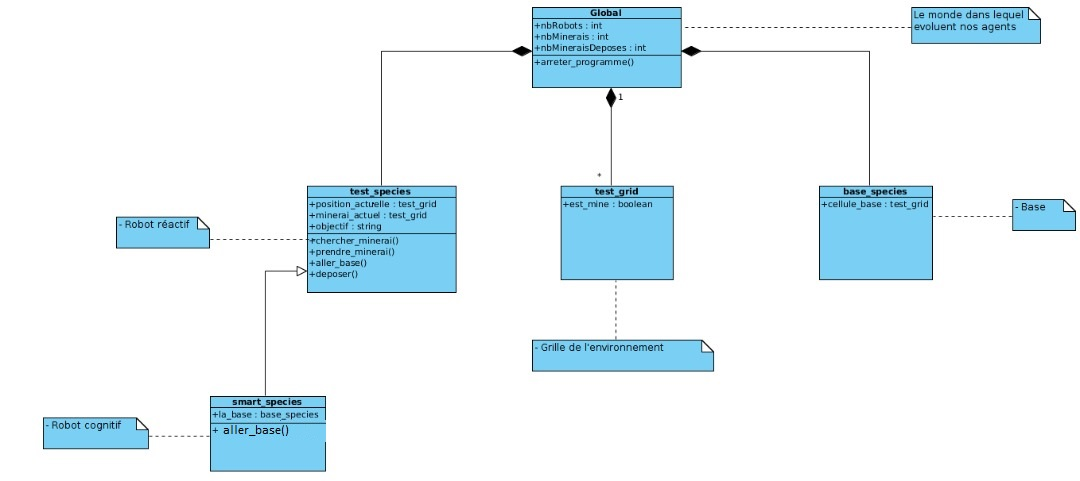
\includegraphics[width=500pt]{diagrammes/diagramme_classe_cognitif}
	\end{center}
	%légende de l'image
	\caption{Réflexe deposer}
\end{figure}

\section{Diagramme d'Activités}

Le diagramme d'activités du Robot Cognitif est le même que celui du robot réactif mis à part le fait que l'activité "Aller à la base" ne se fait pas de la même façon.
\newpage

\subsection{Acheminement des minerais vers la base [Aller a la Base]}

 En effet le déplacement aléatoire ne se fait que lors du premier voyage de transport du minerai vers la base. Après le dépôt le robot sauvegarde les coordonnées de la base pour s'y diriger directement dans le futur. 
 
\begin{figure}[!h]
	\begin{center}
		%taille de l'image en largeur
		%remplacer "width" par "height" pour régler la hauteur
		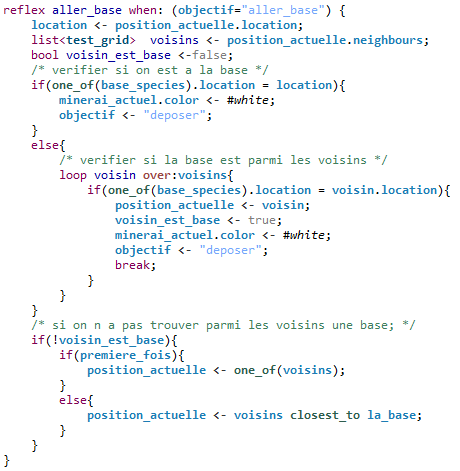
\includegraphics[width=500pt]{code/aller_base_cognitif}
	\end{center}
	%légende de l'image
	\caption{Réflexe aller\_base - Version cognitive}
\end{figure}





\chapter{Tests de Sensibilité}
Dans cette partie nous cherchons à étudier l'évolution du temps de récupération de tous les minerais de l'environnement en fonction du nombre de robots introduits. \\
Le nombre de minerais dans l'environnement est fixé à 40. Étant donné que certains paramètres rentrant en jeu dans l'évaluation de ce temps sont aléatoires (comme exemples, le temps pour aller à la base pour la version réactive, le temps pour trouver la base la première fois pour la version cognitive ou encore le temps pour trouver un minerai), nous répétons la même expérience avec le même nombre de robots un certain nombre de fois (dix ici) et prenons la moyenne des temps des expériences. Cela nous permet d'avoir des valeurs plus fiables. Ensuite, le programme enregistre ces valeurs dans un fichier. Ainsi pour chaque version, un fichier Excel est produit (\textit{reactif.csv} et \textit{cognitif.csv}). Ce sont ces tableaux Excel que nous exploitons par la suite. 

\begin{figure}[!h]
	\begin{center}
		%taille de l'image en largeur
		%remplacer "width" par "height" pour régler la hauteur
		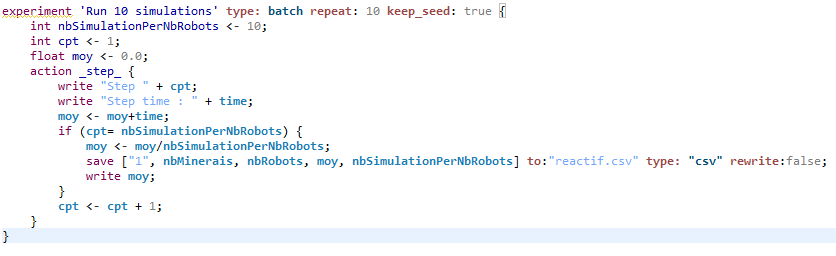
\includegraphics{code/simulations_repetees_reactif}
	\end{center}
	%légende de l'image
	\caption{Simulations répétées de la version réactive}
\end{figure}

\begin{figure}[!h]
	\begin{center}
		%taille de l'image en largeur
		%remplacer "width" par "height" pour régler la hauteur
		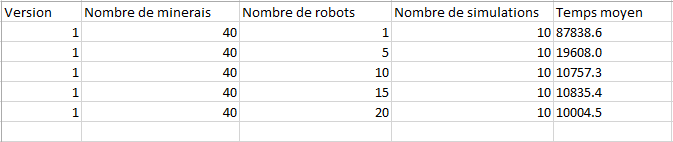
\includegraphics{code/excel_reactif}
	\end{center}
	%légende de l'image
	\caption{Résultat d'exécution des simulations répétées de la version réactive}
\end{figure}

\begin{figure}[!h]
	\begin{center}
		%taille de l'image en largeur
		%remplacer "width" par "height" pour régler la hauteur
		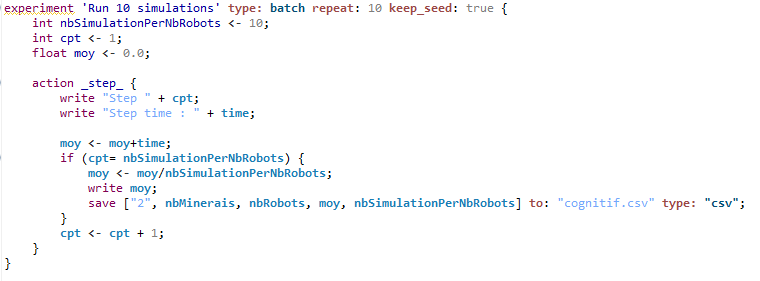
\includegraphics{code/simulations_repetees_cognitif}
	\end{center}
	%légende de l'image
	\caption{Simulations répétées de la version cognitive}
\end{figure}

\begin{figure}[!h]
	\begin{center}
		%taille de l'image en largeur
		%remplacer "width" par "height" pour régler la hauteur
		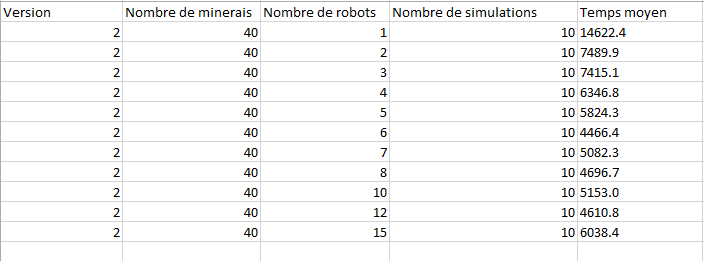
\includegraphics{code/excel_cognitif}
	\end{center}
	%légende de l'image
	\caption{Résultat d'exécution des simulations répétées de la version cognitive}
\end{figure}

\newpage


\section{Robots Réactifs}

%tableau centré à taille variable qui s'ajuste automatiquement suivant la longueur du contenu
\begin{table}[!h]
	\begin{center}
		\begin{tabular}{|r|r|r|r|r|}
			\hline
			Version & Nombre de minerais & Nombre de robots & Nombre de simulations & Temps moyen
			 \\
			\hline
			1 &	40 & 01 & 10 & 87838,6\\
			1 &	40 & 05 & 10 & 19608,0\\
			1 & 40 & 10 & 10 & 10757,3\\
			1 &	40 & 15	& 10 & 10835,4\\
			1 &	40 & 20	& 10 & 10004,5\\
			\hline
		\end{tabular}
	\end{center}
	\caption{Tableau récapitulatif du fichier reactif.csv}
\end{table}
~\\

\begin{center}
\begin{tikzpicture}
\begin{axis}[
	title = {Evolution du temps de récupération des minerais en fonction du nombre de robots - Version réactive},
	xlabel = {Nombre de robots},
	ylabel = {Temps moyen de recuperation},
	xmin=0, xmax=25,
	ymin=0, ymax=88000,
	xmajorgrids = true,
	ymajorgrids = true,
	grid style = dashed
]

\addplot[
color=blue,
]
coordinates {
	(1,87838.6)(5,19608.0)(10,10757.3)(15,10835.4)(20,10004.5)
};

\end{axis}
\end{tikzpicture}
\end{center}

\paragraph*{Interprétation}
~\\
Nous remarquons que le temps moyen de récupération de tous les minerais diminuent au fur et à mesure que l'on ajoute plus de robots. Cependant, à partir de 10 robots, ce temps devient constant.\\
Concrètement, cela veut dire qu'à partir de 10 robots, il ne sert plus à rien d'augmenter le nombre de robots. Cela ne fait que gaspiller des ressources. \\ Aussi, nous notons que le temps optimal pour les robots réactifs tourne autour de 10000 cycles.

\hskip7mm


\section{Robots Cognitifs}

%tableau centré à taille variable qui s'ajuste automatiquement suivant la longueur du contenu
\begin{table}[!h]
	\begin{center}
		\begin{tabular}{|r|r|r|r|r|}
			\hline
			Version & Nombre de minerais & Nombre de robots & Nombre de simulations & Temps moyen \\
			\hline
			2 &	40 & 01 & 10 & 14622,4\\
			2 &	40 & 02 & 10 &  7489,9\\
			2 & 40 & 03 & 10 &  7415,1\\
			2 &	40 & 04	& 10 &  6346,8\\
			2 &	40 & 05	& 10 &  5824,3\\
			2 &	40 & 06	& 10 &  4466,4\\
			2 &	40 & 07	& 10 &  5082,3\\
			2 &	40 & 08	& 10 &  4696,7\\
			2 &	40 & 10	& 10 &  5153,0\\
			2 &	40 & 12	& 10 &  4610,8\\
			2 &	40 & 15	& 10 &  6038,4\\
			\hline
		\end{tabular}
	\end{center}
	\caption{Tableau récapitulatif du fichier cognitif.csv}
\end{table}


\begin{center}
	\begin{tikzpicture}
	\begin{axis}[
	title = {Evolution du temps de récupération des minerais en fonction du nombre de robots - Version cognitive},
	xlabel = {Nombre de robots},
	ylabel = {Temps moyen de recuperation},
	xmin=0, xmax=15,
	ymin=0, ymax=15000,
	xmajorgrids = true,
	ymajorgrids = true,
	grid style = dashed
	]
	
	\addplot[
	color=blue,
	]
	coordinates {
		(1,14622.4)(2,7489.9)(3,7415.1)(4,6346.8)(5,5824.3)(6,4466.4)(7,5082.3)(8,4696.7)(10,5153.0)
		(12,4610.8)
	};
	
	\end{axis}
	\end{tikzpicture}
\end{center}

\paragraph*{Interprétation}
~\\
Ici aussi, nous remarquons que le temps moyen de récupération de tous les minerais diminuent au fur et à mesure que l'on ajoute plus de robots. Cependant, ici dès qu'on atteint 6 robots, ce temps devient presque constant.\\
A partir de 6 robots, il n'est plus nécessaire d'ajouter des robots\\ Aussi, nous notons que le temps optimal pour les robots cognitifs tourne autour de 5000 cycles.
\hskip7mm

\section{Version réactive \textit{vs} Version cognitive}

\begin{table}[!h]
	\begin{center}
		\begin{tabular}{|l|r|r|r|}
			\hline
			Version & Nombre de minerais & Nombre de robots & Temps moyen \\
			\hline
			Réactive   & 40 & 01 & 87838,6\\
			Cognitive  & 40 & 01 & 14622,4\\
			\hline
		\end{tabular}
	\end{center}
	\caption{Temps de résolution pour un robot de chaque version}
\end{table}

\begin{align*}
\frac{87838,6}{14622,4} = 6, 0071\\
\end{align*}
Nous remarquons qu'un robot cognitif met approximativement 6 fois moins de temps à récupérer tous les minerais qu'un robot réactif.

\begin{center}
	\begin{tikzpicture}
	\begin{axis}[
	title = {Comparaison des temps de récupération des minerais en fonction du nombre de robots},
	xlabel = {Nombre de robots},
	ylabel = {Temps moyen de recuperation},
	xmin=0, xmax=25,
	ymin=0, ymax=88000,
	xmajorgrids = true,
	ymajorgrids = true,
	grid style = dashed,
	axis x line=bottom,
	axis y line=left
	]
	
	\addplot[mark=none,red,thick] coordinates {
		(1,87838.6)(5,19608.0)(10,10757.3)(15,10835.4)(20,10004.5)
	};
	\addlegendentry{Version réactive}
	\addplot[mark=none,blue,thick] coordinates {
		(1,14622.4)(2,7489.9)(3,7415.1)(4,6346.8)(5,5824.3)(6,4466.4)(7,5082.3)(8,4696.7)(10,5153.0)
		(12,4610.8)
	};
	\addlegendentry{Version cognitive}
	\end{axis}
	\end{tikzpicture}
\end{center}
De même, nous remarquons que pour atteindre le temps optimal pour la version réactive, il nous faut introduire jusqu'à 10 robots alors que pour la version cognitive ce temps est atteint à partir de 6 robots. Aussi, à temps optimaux et nombres de robots optimaux, la version cognitive est 2 fois plus rapides (5000 cycles contre 10000 pour la version réactive).\\
Néanmoins, il faut noter que la version cognitive est plus gourmande en ressources alors que la version réactive consomme peu de ressources.\\
Ainsi, nous voyons que chaque version est adapté à une situation bien déterminée. En effet, si on a la possibilité d'avoir plusieurs et que l'on est limité en ressources, il est préférable d'utiliser la version réactive alors que si on est dans une situation ou les ressources ne constituent pas une contrainte, il est plus judicieux d'utiliser la version cognitive qui nous permet d'être plus efficace.


\renewcommand{\abstractnamefont}{\normalfont\Large\bfseries}
%\renewcommand{\abstracttextfont}{\normalfont\Huge}
\renewcommand{\abstractname}{Conclusion}

\begin{abstract}
\hskip7mm

\begin{spacing}{1.3}

Dans cette étude de cas, nous étions face à la situation : l'exploitation d'un territoire minier par une population de robots. Pour y apporter des réponse, nous avons produits deux version de robot. Une dite réactive et une autre un peu plus "intelligente" dite cognitive. Nous avons vu que chacune de ces versions était adapté à une situation précise avec ses forces et faiblesses. Et si on faisait travailler ensemble ces deux types de robot ? Voilà une question qui mériterait d'être étudiée.

\end{spacing}
\end{abstract}


%page blanche
\newpage
~
%ne pas numéroter cette page
\thispagestyle{empty}
\newpage

\renewcommand{\listfigurename}{List des figures}

\renewcommand{\listtablename}{Liste des Tables}


\thispagestyle{empty}

\listoffigures

\listoftables

\clearpage

\pagenumbering{arabic}

%page blanche
\newpage
~
%ne pas numéroter cette page
\thispagestyle{empty}
\newpage



\end{document}